\documentclass{article}

\newcommand{\order  }{{\cal O}}
\newcommand{\mc     }{\mathcal}
\newcommand{\bra    }{\langle}
\newcommand{\ket    }{\rangle}
\newcommand{\Bra    }{\left\langle}
\newcommand{\Ket    }{\right\rangle}
\newcommand{\atanh  }{{\rm{atanh}}}
\newcommand{\sech   }{\mathrm{sech}}

\newcommand{\bA     }{\mbox{\boldmath$A$}}
\newcommand{\bB     }{\mbox{\boldmath$B$}}
\newcommand{\bC     }{\mbox{\boldmath$C$}}
\newcommand{\bD     }{\mbox{\boldmath$D$}}
\newcommand{\bE     }{\mbox{\boldmath$E$}}
\newcommand{\bF     }{\mbox{\boldmath$F$}}
\newcommand{\bG     }{\mbox{\boldmath$G$}}
\newcommand{\bH     }{\mbox{\boldmath$H$}}
\newcommand{\bI     }{\mbox{\boldmath$I$}}
\newcommand{\bJ     }{\mbox{\boldmath$J$}}
\newcommand{\bK     }{\mbox{\boldmath$K$}}
\newcommand{\bL     }{\mbox{\boldmath$L$}}
\newcommand{\bM     }{\mbox{\boldmath$M$}}
\newcommand{\bN     }{\mbox{\boldmath$N$}}
\newcommand{\bO     }{\mbox{\boldmath$O$}}
\newcommand{\bP     }{\mbox{\boldmath$P$}}
\newcommand{\bQ     }{\mbox{\boldmath$Q$}}
\newcommand{\bR     }{\mbox{\boldmath$R$}}
\newcommand{\bS     }{\mbox{\boldmath$S$}}
\newcommand{\bT     }{\mbox{\boldmath$T$}}
\newcommand{\bU     }{\mbox{\boldmath$U$}}
\newcommand{\bV     }{\mbox{\boldmath$V$}}
\newcommand{\bW     }{\mbox{\boldmath$W$}}
\newcommand{\bX     }{\mbox{\boldmath$X$}}
\newcommand{\bY     }{\mbox{\boldmath$Y$}}
\newcommand{\bZ     }{\mbox{\boldmath$Z$}}

\newcommand{\ba     }{\mbox{\boldmath$a$}}
\newcommand{\bb     }{\mbox{\boldmath$b$}}
\newcommand{\bc     }{\mbox{\boldmath$c$}}
\newcommand{\bd     }{\mbox{\boldmath$d$}}
\newcommand{\be     }{\mbox{\boldmath$e$}}
%\newcommand{\bf     }{\mbox{\boldmath$f$}}
\newcommand{\bg     }{\mbox{\boldmath$g$}}
\newcommand{\bh     }{\mbox{\boldmath$h$}}
\newcommand{\bi     }{\mbox{\boldmath$i$}}
\newcommand{\bj     }{\mbox{\boldmath$j$}}
\newcommand{\bk     }{\mbox{\boldmath$k$}}
\newcommand{\bl     }{\mbox{\boldmath$l$}}
\newcommand{\bm     }{\mbox{\boldmath$m$}}
\newcommand{\bn     }{\mbox{\boldmath$n$}}
\newcommand{\bo     }{\mbox{\boldmath$o$}}
\newcommand{\bp     }{\mbox{\boldmath$p$}}
\newcommand{\bq     }{\mbox{\boldmath$q$}}
\newcommand{\br     }{\mbox{\boldmath$r$}}
\newcommand{\bs     }{\mbox{\boldmath$s$}}
\newcommand{\bt     }{\mbox{\boldmath$t$}}
\newcommand{\bu     }{\mbox{\boldmath$u$}}
\newcommand{\bv     }{\mbox{\boldmath$v$}}
\newcommand{\bw     }{\mbox{\boldmath$w$}}
\newcommand{\bx     }{\mbox{\boldmath$x$}}
\newcommand{\by     }{\mbox{\boldmath$y$}}
\newcommand{\bz     }{\mbox{\boldmath$z$}}


\newcommand{\blambda}{\mbox{\boldmath$\lambda$}}
\newcommand{\bkappa }{\mbox{\boldmath$\kappa$}}
\newcommand{\bXI    }{\mbox{\boldmath$\Xi$}}
\newcommand{\bLAMBDA}{\mbox{\boldmath$\Lambda$}}
\newcommand{\balpha}{\mbox{\boldmath$\alpha$}}
\newcommand{\bbeta}{\mbox{\boldmath$\beta$}}


\newcommand{\bGAMMA }{\mbox{\boldmath$\Gamma$}}
\newcommand{\bSigma }{\mbox{\boldmath$\Sigma$}}
\newcommand{\bsigma }{\mbox{\boldmath$\sigma$}}
\newcommand{\bdeltaL}{\mbox{\boldmath$\delta L$}}
\newcommand{\bone   }{\mbox{\boldmath$1$}}
\newcommand{\bomega }{\mbox{\boldmath$\omega$}}
\newcommand{\boldeta}{\mbox{\boldmath$\eta$}}
\newcommand{\btau   }{\mbox{\boldmath$\tau$}}
\newcommand{\bpsi   }{\mbox{\boldmath$\psi$}}
\newcommand{\bzero  }{\mbox{\boldmath$0$}}

\newcommand{\bphi   }{\mbox{\boldmath$\phi$}}
\newcommand{\bxi    }{\mbox{\boldmath$\xi$}}
\newcommand{\bhxi   }{\mbox{\boldmath$\hat{\xi}$}}
\newcommand{\bzeta  }{\mbox{\boldmath$\zeta$}}
\newcommand{\tr     }{\textnormal{tr}\:}
\newcommand{\Tr     }{\textnormal{Tr}\:}
\newcommand{\limN}{\underset{N\rightarrow \infty}{\textnormal{lim}}}
\newcommand{\atilde}{\tilde{a}}
\usepackage{amsmath}
\usepackage{amssymb}
\usepackage{amstext}
\usepackage{amsfonts}
\usepackage{graphicx}
\usepackage{epsfig}
\usepackage{subfig}
\usepackage{xcolor}
\usepackage{rotating}
\usepackage{soul}
\usepackage{hyperref}
\usepackage{adjustbox}

\newlength\myheight

\usepackage{spconf,amsmath,epsfig}
\usepackage{graphicx}
\usepackage{epsfig}
\usepackage{subfig}
\usepackage{xcolor}
\usepackage{amsmath}
\newcommand\norm[1]{\left\lVert#1\right\rVert}
\usepackage{listings}
\usepackage[ruled,vlined,linesnumbered]{algorithm2e}
\usepackage{cite}
\usepackage{fixltx2e}
\usepackage{xcolor}
\usepackage{subfig}
\usepackage{amssymb}
\usepackage{times}
\usepackage{fancyhdr,graphicx,amsmath,amssymb}
\usepackage[ruled,vlined]{algorithm2e}


% Title.
% ------
\title{Sparse spectral unmixing using a group nuclear norm}
%
% Single address.
% ---------------
\name{Vera Andrejchenko, Marina Ljubenovic, Paul Scheunders
}
\address{Imec-Visionlab, University of Antwerp\\
Universiteitsplein 1, Building N \\
B-2610 Wilrijk (Antwerp), Belgium \\
}

\begin{document}
%\ninept
%
\maketitle
%
\begin{abstract}
In hyperspectral images the observed spectra generally appear as mixtures of %in mixtures of 
pure materials (endmembers). Sparse unmixing methods aim to recover the abundances of these materials, taking prior information into account e.g. the limitation of the number of pure signatures in the mixtures, the spatial homogeneity of the pixels or availability and contribution of multiple endmembers (groups) per material. In this work, we will incorporate all of the above simultaneously, i.e. we will address the spatially homogeneity, the limited contribution from groups of endmembers i.e. between group sparsity, the similarity of the abundances within the groups i.e. withing group sparsity. This will be done by defining an optimization function based on nuclear norm relaxation. Quantitative and qualitative experiments on synthetic data show the potential of our approach.    
%utilize the multiple endmembers per group, 
\end{abstract}
%
\begin{keywords}
hyperspectral unxming, low rank 
\end{keywords}
%
\section{Introduction}
In hyperspectral images, the observed spectra can be regarded as mixtures of pure materials, from which the spectra can be obtained from a spectral library,   acquired from pure pixels in the image, or acquired from the ground. In order to distinguish between these pure materials (endmembers) and find their abundances  within the mixed pixels, spectral unmixing methods were developed. Methods that represent the mixed spectra as linear combinations of endmembers, imposing pixelwise abundance sparsity, i.e. forcing only a limited number of materials to be present in the mixture are widely used \cite{spUnmix}. On the other hand,  collaborative sparse unmixing methods enforce joint sparsity among all the pixels, assuming that a small number of endmembers is present in the entire image. These methods produce only a few nonzero rows in the abundance matrix, corresponding to pixels sharing the same active set of endmembers \cite{iordache14}.
Other methods impose structured group sparsity, in which the endmembers %appear in groups 
are organized in groups (several endmembers per material). The abundance values associated with these endmembers are also organized in groups. These methods aim to obtain sparsity across and within the abundance groups at per-pixel level \cite{spGroup_unmix},\cite{socialSparsity}. An approach that accounts for  spatial homogeneity enforces similarity of abundances
and their smooth transitions is SunSAL-TV \cite{totVar}.

While the current methods consider only certain aspects and perform the unmixing in a pixel-wise and independent manner, including either spatial or group information, in our work we attempt to address all aspects in a simultaneous way. We present a method that simultaneously considers: 1) the availability of multiple endmembers per material, organized in groups, all being able to contribute to the description of the mixtures, 2) a limitation on the groups of materials present in the mixture, resulting in between-group sparsity, 3) a limitation on the number of endmembers contributing per group along with the exploitation of the similarity of abundances within a group, producing within-group sparsity, 4) the exploitation of (local) spatial variation of neighboring pixels, producing spatially homogeneous neighboring abundances.
We accomplish this by employing the low rank nature of the abundances of neighboring pixels 
and exploit the fact that the abundances within a group are highly correlated. 
Thus we focus on both the spatial and group information at the same time.
\section{Method}
In this paper, we model the observed spectra: $\bY \in \mathbb{R}^{m \times n}$ following the linear mixing model: 
\begin{eqnarray}
\mathbf{Y}= \mathbf{E}\mathbf{A} + \mathbf{n}
\end{eqnarray}
with $m$ the number of bands and $n$ the number of observed spectra. 
This model assumes that the observed spectrum is a linear combination of pure materials - endmembers. The endmember matrix: $\bE \in \mathbb{R}^{m \times p}$ is assumed to be known and structured in groups: $j = 1...G$, such that it contains several endmembers per material, where $p = p_1 + p_2 + ... p_G$, with $p_j$ being the number of endmembers for group $j$. 
$\bA \in \mathbb{R}^{p \times n}$ is the matrix with fractional abundances for the grouped endmembers and $\mathbf{n}$ the additive noise. 
To address the above mentioned aspects and
leverage the fact that the  available endmember set is organized in groups we propose the following unmixing method:
\begin{eqnarray} 
\label{eqn:obj}
\min_{A} \frac{1}{2} \| \bE \bA -\bY \|_F^2 +\lambda\| \bH\bA \|_{1,G,*}  \\
\quad s.t. \bA \geq 0  \nonumber
\end{eqnarray} 
\begin{figure}[h]   
	\captionsetup[subfigure]{labelformat=empty,font=small}
	\settoheight\myheight{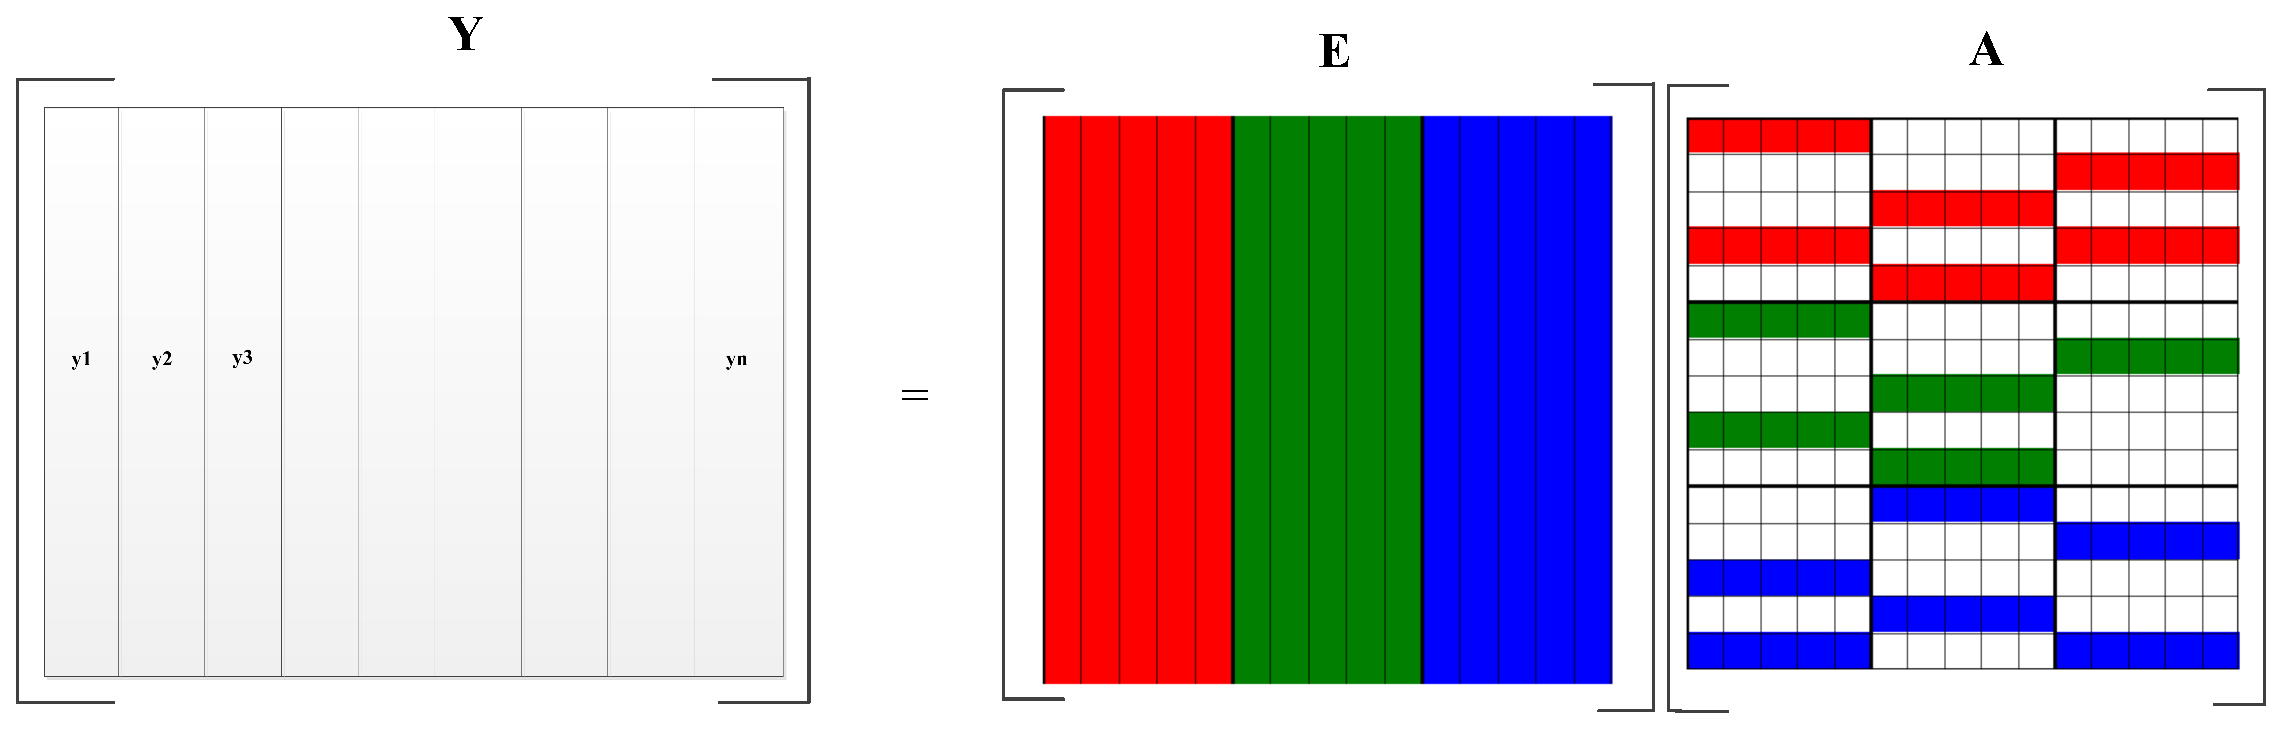
\includegraphics[width=0.45\textwidth]{./images/method/eps/python_group_nuclear_formula.eps}}
	\centering
	\subfloat[]{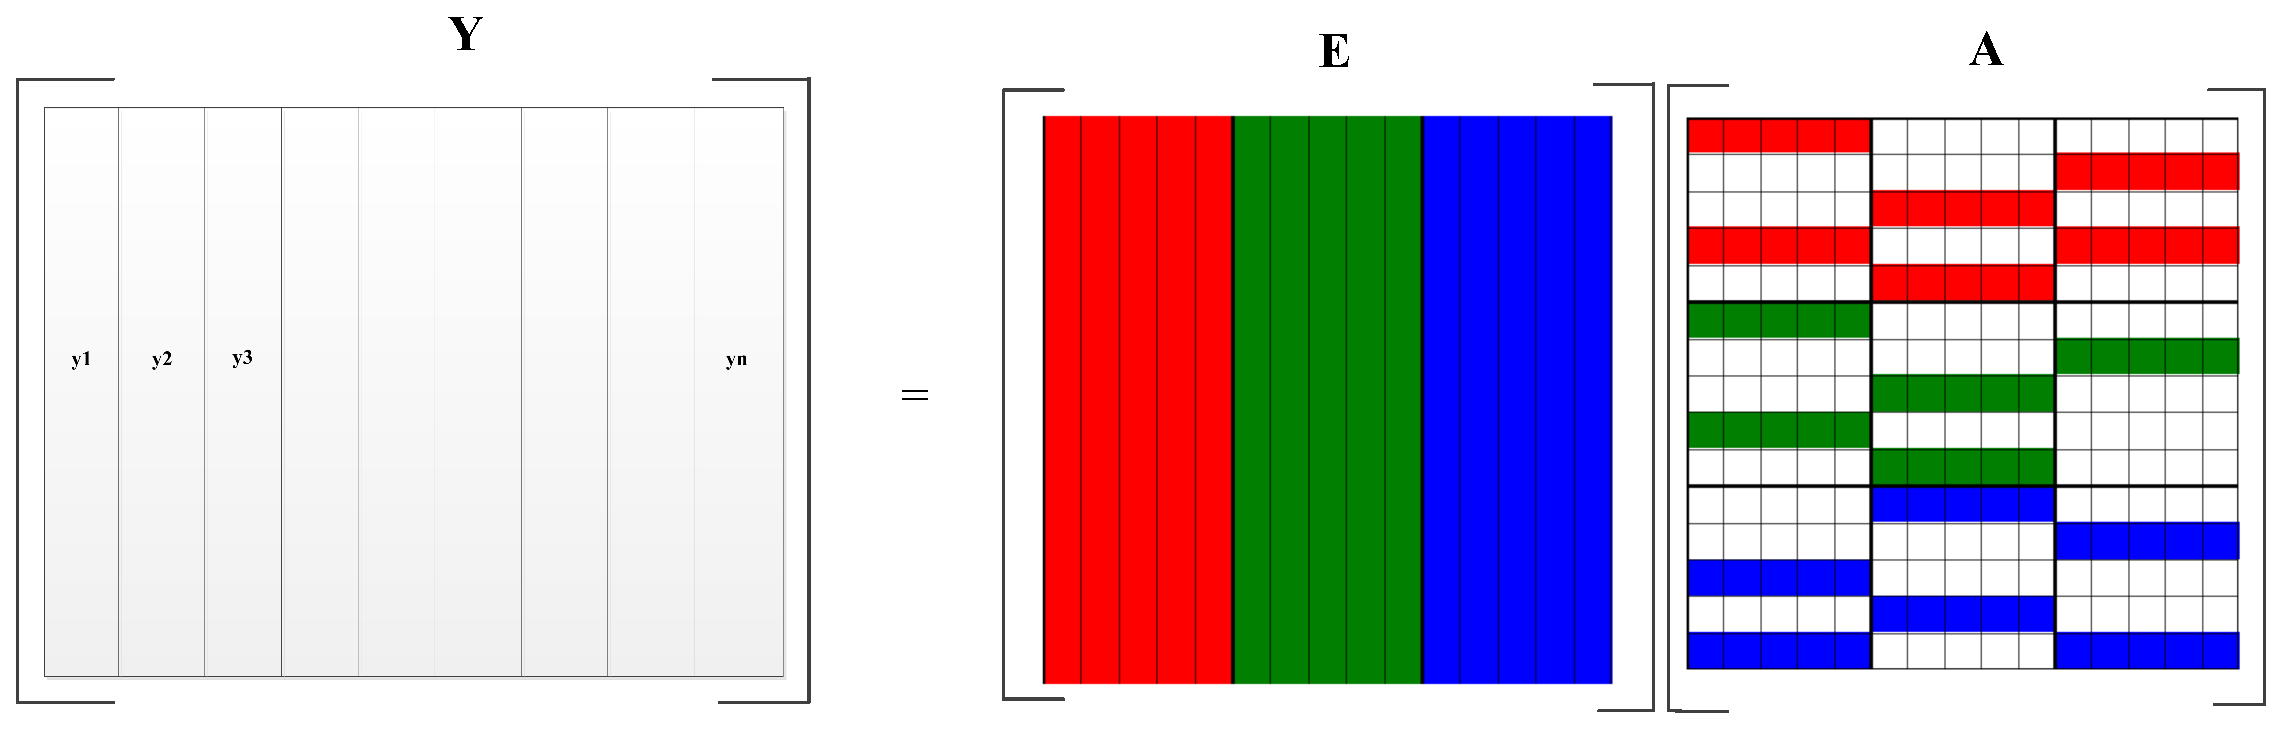
\includegraphics[height=\myheight]{./images/method/eps/python_group_nuclear_formula.eps}} \hspace{1mm} 
	\caption{Graph illustration of the proposed method. Endmembers from the same group have the same color. Active endmembers in $\bA$ are colored, non-active endmembers are white. Neighbourhood and grouping is represented by big squares with thicker sides. 
}
\label{BuildingParameters}
\end{figure}
\\ using the $l_{1,G,*}$ mixed norm: \\ $\|  \bH\bA \|_{1,G,*} \equiv \sum_{i=1}^n{\sum_{j = 1}^{G}{\|\bH_j\bA_{\mathcal{N}_{(i)}}}\|_*} $, where $\bH_j \in \mathbb{R}^{p_j \times p}$ is the selector matrix for group $j$, with $\mathcal{N}_{(i)}$ the neighborhood of the $i$-th pixel,  $\bH_j\bA_{\mathcal{N}_{(i)}}$  being the abundances from group $j$ associated with the abundances of neighboring pixels $\mathcal{N}_{(i)}$. Note that we enforce square sub-matrices such that the size of the neighborhood should equal the number of elements in each group. The nuclear norm: $\| \mathord{\cdot} \|_*$,  which is a convex relaxation of the rank of a matrix, is applied on each square sub-matrix: $\bH_j\bA_{\mathcal{N}_{(i)}}$, and is defined as: $\| \bH_j\bA_{\mathcal{N}_{(i)}} \|_* = \sum_{k}{\sigma_k(\bH_j\bA_{\mathcal{N}_{(i)}})}$, where $\sigma_k(\bH_j\bA_{\mathcal{N}_{(i)}})$  are the singular values of $\bH_j\bA_{\mathcal{N}_{(i)}}$.
Due to the high similarity of the abundances of neighboring pixels and at the same time the high correlation of abundances within a group, these abundance sub-matrices have a low rank. So $\| \mathord{\cdot} \|_*$   
is there to enforce the low rank structure of: $ \bH_j\bA_{\mathcal{N}_{(i)}}$. 
The parameter $\lambda$ is the regularization parameter for the group nuclear norm. An equivalent formulation of the above problem is given by: 
\begin{gather}
\label{eqn:obj}
\min_{A} \frac{1}{2} \| \bE \bA -\bY \|_F^2 +\lambda\| \bH\bA \|_{1,G,*}  + l_{R_+}{(\bA)}
\end{gather}
with $l_{R_+}{(\bA)}$ being the indicator function, applied on the columns of $\bA$: $\balpha_i$, being 0 if $\balpha_i$ belongs to the nonnegative orthant and $+\infty$ otherwise.

We introduce a set of new variables ($\bV_1, .... \bV_{j},..\bV_{G},\\ \bV_{G+1},\bV_{G+2}$, for $j = 1..G$ and their corresponding Lagrange multipliers $\bD_j$) for each constraint, as well as an internal penalty parameter $\mu$. %regularizer 
The $\bV_j$s with  $j = 1..G$ are the variables associated with the groups of $\bA$, whereas the $\bV_{G+1}$ and $\bV_{G+2}$ with the entire $\bA$ matrix.
Afterwards we construct the augmented lagrangian $\mathcal{L}$ (\ref{eq:lagrangian}) and use the alternating direction method of multipliers (ADMM)\cite{admm} to solve the optimization problem. 
\begin{gather} \label{eq:lagrangian}
\mathcal{L} = \frac{1}{2}\| \bV_{G+1} - \bY \|_F^2 + l_{R_+}{(\bV_{G+2})} + \lambda \sum_{j=1}^G{\| \bV_j\|_*} \\ \nonumber
+ \frac{\mu}{2}\| \bE\bA - \bV_{G+1} - \bD_{G+1}\|_F^2 + \frac{\mu}{2}\| \bA - \bV_{G+2} - \bD_{G+2}\|_F^2 +         \\ \nonumber
\frac{\mu}{2}\sum_{j=1}^G{\|\bH_j\bA  - \bV_j - \bD_j\|_F^2} 
\end{gather}
Algorithm1 depicts the ADMM algorithm for our optimization problem, which optimizes $\mathcal{L}$ w.r.t. all variables and updates the Lagrange multipliers  $\bD_j$.
\begin{algorithm}[h!]
\SetAlgoLined
\KwResult{$\hat{\bA}$}
 initialization: set  \scalebox{0.8}{$k = 0$, $\mu>0$, $\bA_0, \bV_0,...\bD_0$}   \;
 \While{\scalebox{0.8}{While stopping criterion is satisfied}}{
  \scalebox{0.8}{$\bA^{k+1}   = \arg \min_A \mathcal{L}(\bA, \bV_{1:(G+2)}^{k}, \bD_{1:(G+2)}^{k} )$} \\ 
  \For{ \scalebox{0.8}{$j = 1..G$}}{ 
  		\For{ \scalebox{0.8}{$i = 1..n$}}{ 
  			\scalebox{0.8}{$\mathcal{N}_{(i)}<-get\_Neighbours(i)$} \\
        	\scalebox{0.8}{$\bV_{j,\mathcal{N}_{(i)}}^{k+1}$ =  Prox$^{*}(\bH_j\bA_{\mathcal{N}_{(i)}}^{k+1} - \bD_{j,\mathcal{N}_{(i)}}^{k}, \frac{\lambda}{\mu})   $}	
        }
        \scalebox{0.8}{$\bD_j^{k+1}$ = $\bD_j^k -  (\bH_j\bA^{k+1} - \bV_j^{k+1})  $}
   }
      \scalebox{0.8}{$\bV_{G+1}^{k+1} =  \arg \min_{V_{G+1}} \mathcal{L}(\bA^{k+1}, \bV_{1:G}^{k}, \bV_{G+1}, \bV_{G+2}^k, \bD_{1:(G+2)}^{k} )$}  \\
  \scalebox{0.8}{$\bV_{G+2}^{k+1} =  \arg \min_{V_{G+2}} \mathcal{L}(\bA^{k+1}, \bV_{1:(G+1)}^{k}, \bV_{G+2}, \bD_{1:(G+2)}^{k} ) $}  \\  
  \scalebox{0.8}{$\bD_{(G+1)}^{k+1}$ = $\bD_{(G+1)}^k -  (\bE\bA^{k+1} - \bV_{(G+1))}^{k+1})  $}
  \scalebox{0.8}{$\bD_{(G+2)}^{k+1}$ = $\bD_{(G+2)}^k -  (\bA^{k+1} - \bV_{(G+2)}^{k+1})  $}
 }
 \caption{ADMM for solving the problem (3)}
\end{algorithm}
The iteration procedure is stopped when the  primal residual norms become smaller than a certain $\epsilon$.
The objective function contains the nuclear norm reqularizer: $\| \mathord{\cdot} \|_*$, which is a non-smooth function. Therefore we resort to proximal methods, which deal with non-differentiable functions by introducing the notion of proximal operators \cite{proxAlgo} associated to a regularizer, which is the nuclear norm in our case. Thus in order to obtain the solution for $\bV_j$ in line 7, for our regularizer we use the singular values soft thresholding proximal operator: $\mathbf{Prox}^*_{\tau}(\bH_j\bA_{\mathcal{N}_{(i)}}) = \bU\mathbf{\Sigma}_{\tau}\bW^T$ where $\mathbf{\Sigma}_{\tau} = diag([(\sigma_1 - \tau)_+,(\sigma_2 - \tau)_+, ...])$ and $\tau = \frac{\lambda}{\mu}$ (note: this soft thresholding of the singular values of a matrix reduces the rank even further). %Prox$^*_{\tau}(\bX) = \sum_{i=1}^{n}{(\sigma_i - \tau)_{+}u_iv_i^T}$. 
The $\mathbf{Prox}^*_{\tau}(\cdot)$ operator is applied on sub-matrix structures: $\bH_j\bV_{\mathcal{N}_{(i)}}$ with $ \mathcal{N}_{(i)}$ the neighborhood of pixel $i$ for a specific group $j$: 
%\begin{equation}
%\mathbf{Soft}^*_{\tau}(\bV) = 
%\begin{bmatrix}
%    \mathbf{Soft}^*_{\tau}{(\bV_{\mathcal{N}_{(i)},1})} & \dots &  \mathbf{Soft}^*{\tau}{(\bV_{\mathcal{N}_{(n)},1})} \\
%     \vdots & \vdots & \vdots   \\
%    \mathbf{Soft}^*_{\tau}{(\bV_{\mathcal{N}_{(i)},j})} & \dots &  \mathbf{Soft}^*{\tau}{(\bV_{\mathcal{N}_{(n)},j})}   \\
%    \vdots & \vdots & \vdots  \\
%      \mathbf{Soft}^*_{\tau}{(\bV_{\mathcal{N}_{(i)},j})} & \dots &  \mathbf{Soft}^*{\tau}{(\bV_{\mathcal{N}_{(n)},G})} 
%\end{bmatrix} 
%\nonumber
%\end{equation}
where $i \in {1..n}$ and $j \in {1..G}$.
Soft-thresholding of the singular values of these sub-matrices  encourages them to be sparse i.e. to have low rank.   
\section{EXPERIMENTS AND RESULTS}
\subsection{Simulated data cubes}
We have generated four different simulated hyperspectral cubes using endmembers from the USGS spectral library \footnote{\href {http://speclab.cr.usgs.gov/spectral.lib06}{http://speclab.cr.usgs.gov/spectral.lib06}}. We selected 33 minerals and then picked 25 spectra from each mineral. For those minerals which had insufficient spectra (less than 25 signatures) we artificially generated the necessary spectra by taking linear combinations of the available spectra for that specific mineral. The very high correlation of the original endmembers within the mineral groups justifies this endmember generation approach. The fractional abundances of these endmembers were selected from a uniform distribution in the range $[0-1]$ and were then normalized to sum to 1. We generated the observed spectra with dimensions: 40 $\times$ 60 pixels and 51 bands, using the linear mixture model and we additionally added white Gaussian noise with signal-to-noise ratio (SNR) of 30 dB. For each pixel from the hyperspectral cube, we associated an abundance vector of 825 elements (33 groups $\times$ 25 elements per groups) and placed these abundance vectors in an abundance cube with dimensions: 40 $\times$ 60 $\times$ 825, see Figure: \ref{genA} a).
In order to mimic the real life (local) spatial homogeneity of the observed spectra, where neighboring pixels have similar abundance values, we first divided the abundance cube into segments of size: 20 $\times$ 20 $\times$ 825.  Furthermore, we added spatial correlation to the abundance cube by 
spatially filtering the cube with a 2D Gaussian kernel ($\sigma = 2$), segment by segment, see Figure: \ref{genA} b). 
Moreover, for each group we applied 1D low-pass filtering with bandwidth 2 of the abundance values in the abundance direction %to the abundances 
in order to simulate correlation of the abundances within the same group (see Figure: \ref{genA} c). To simulate that only certain groups of the endmembers/minerals contribute to the observed spectrum, we randomly set a limited number of groups to be active, and force a limited number of elements within the active group to be non-zero (see Figure: \ref{genA} d). In this way, we introduced sparsity over groups and within groups, as well as spatially correlated abundances and correlation of the abundance values in the abundance direction.
We created the following datasets: 1) Cube1 - only one group of endmembers is active and only one element within that group is active, 2) Cube2 - one group of endmembers is active and two elements within that group are active, 3) Cube3 - two groups of endmembers are active and only one element within each group is active, 4) Cube4 - two groups of endmembers are active and two elements within the groups are active. 
\begin{figure}[h!]
	\captionsetup[subfigure]{labelformat=empty,font=small}
	\settoheight\myheight{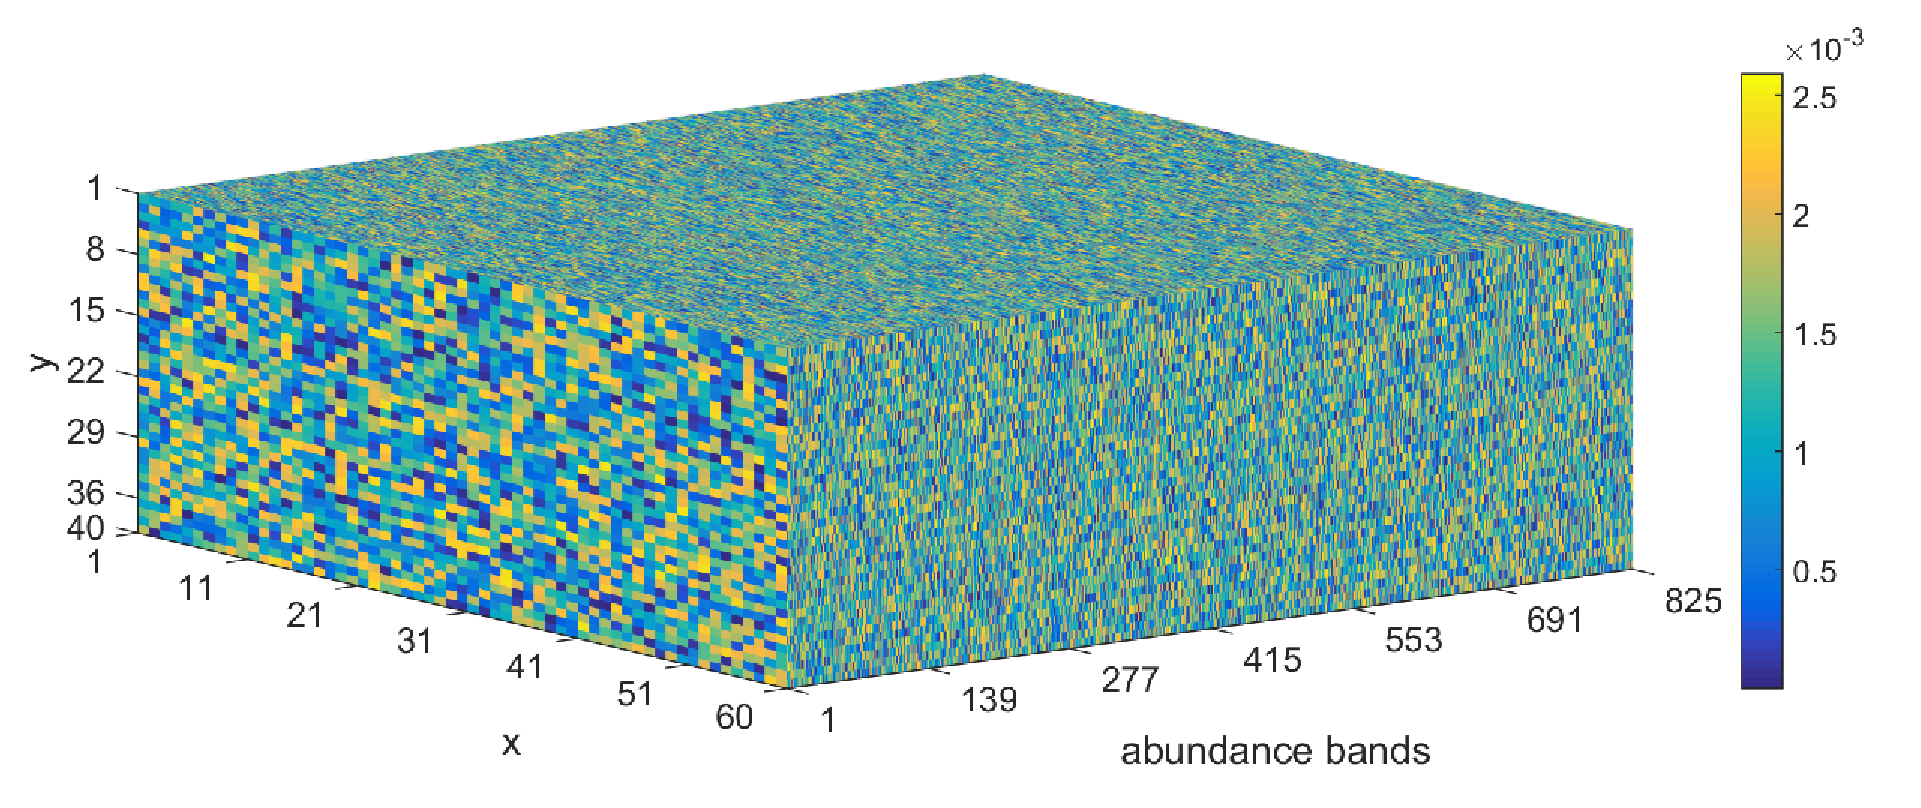
\includegraphics[width=0.30\textwidth]{./images/generated_A/1.eps}}
	\centering
	\subfloat[a)]{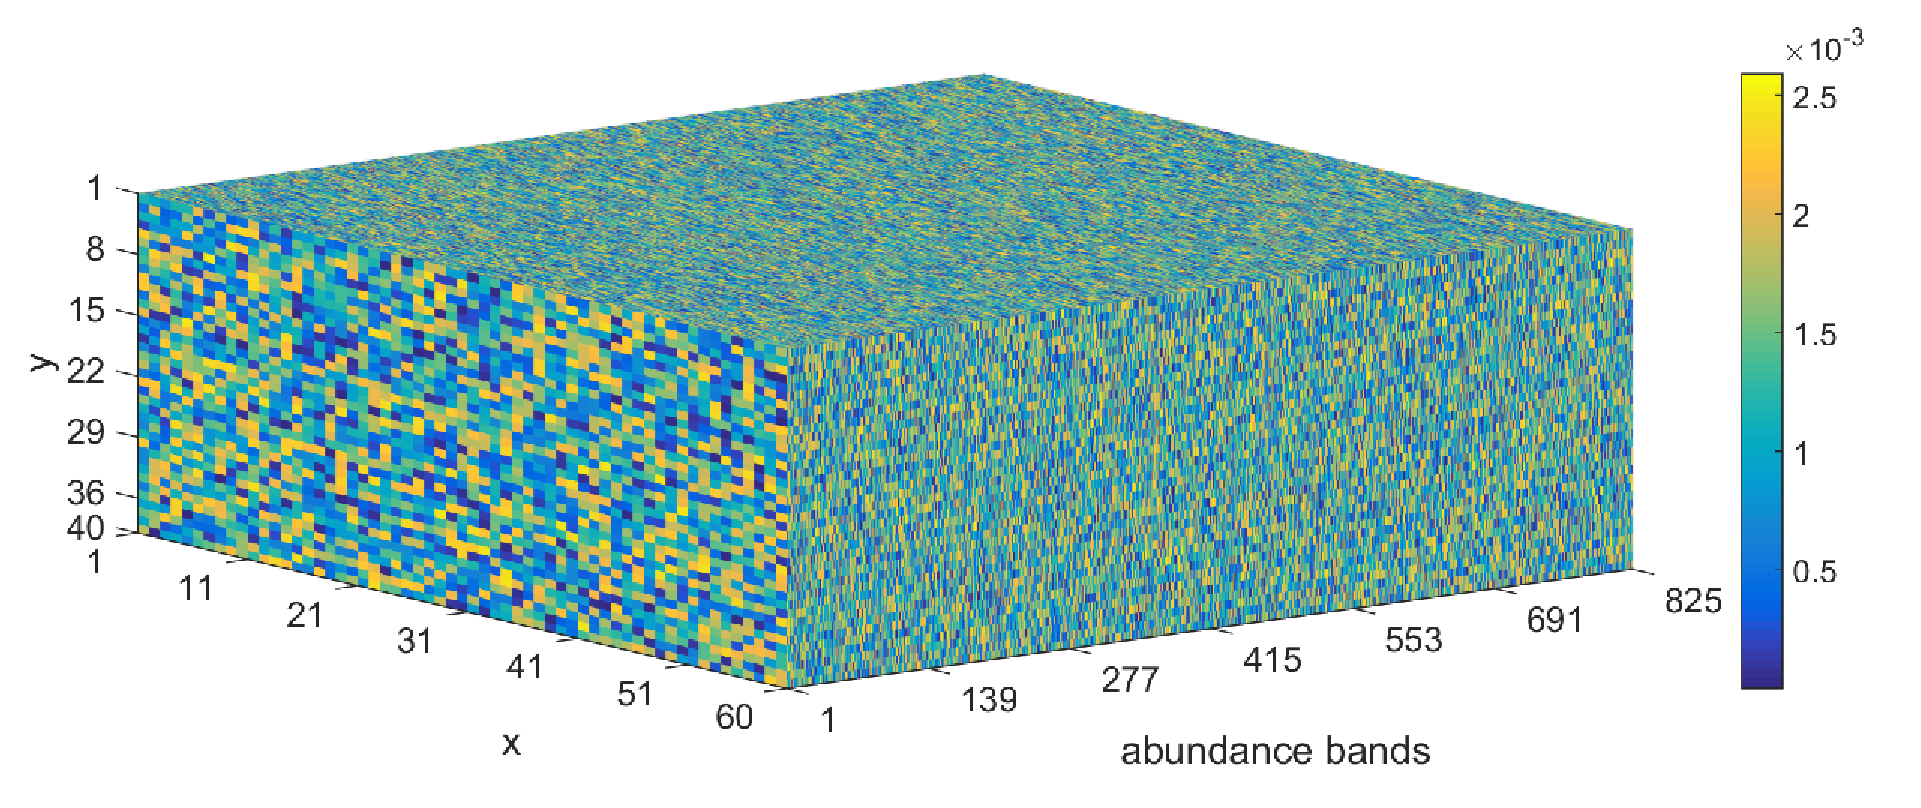
\includegraphics[height=\myheight]{./images/generated_A/1.eps}} \hspace{1mm} 
	\subfloat[b)]{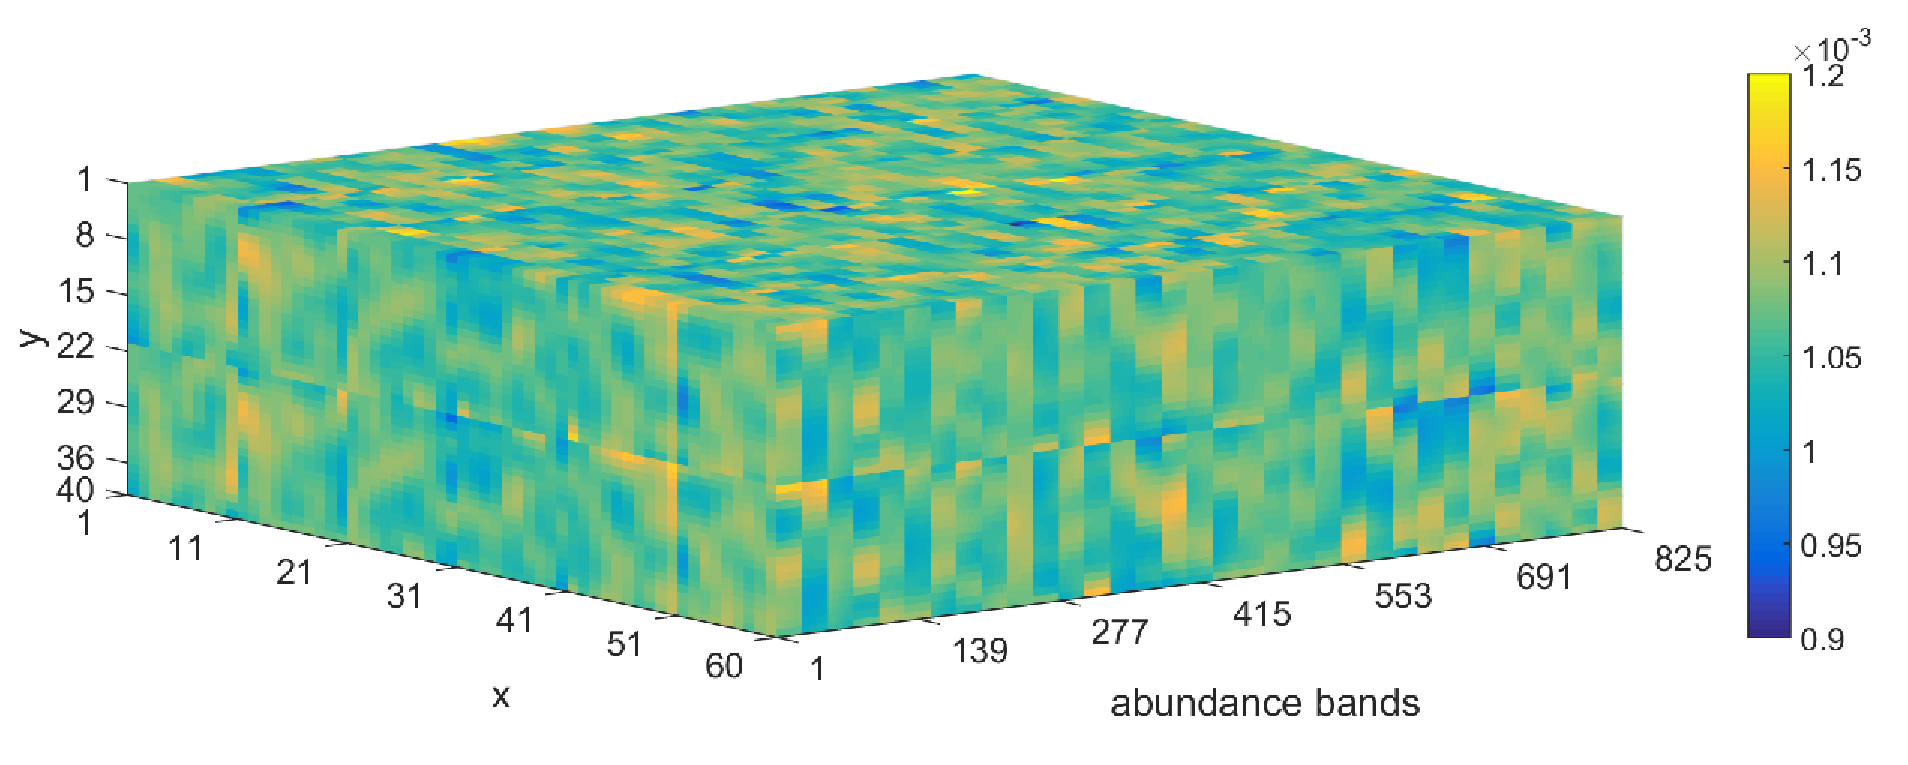
\includegraphics[height=\myheight]{./images/generated_A/2.eps}} \hspace{1mm} \\
	\subfloat[c)]{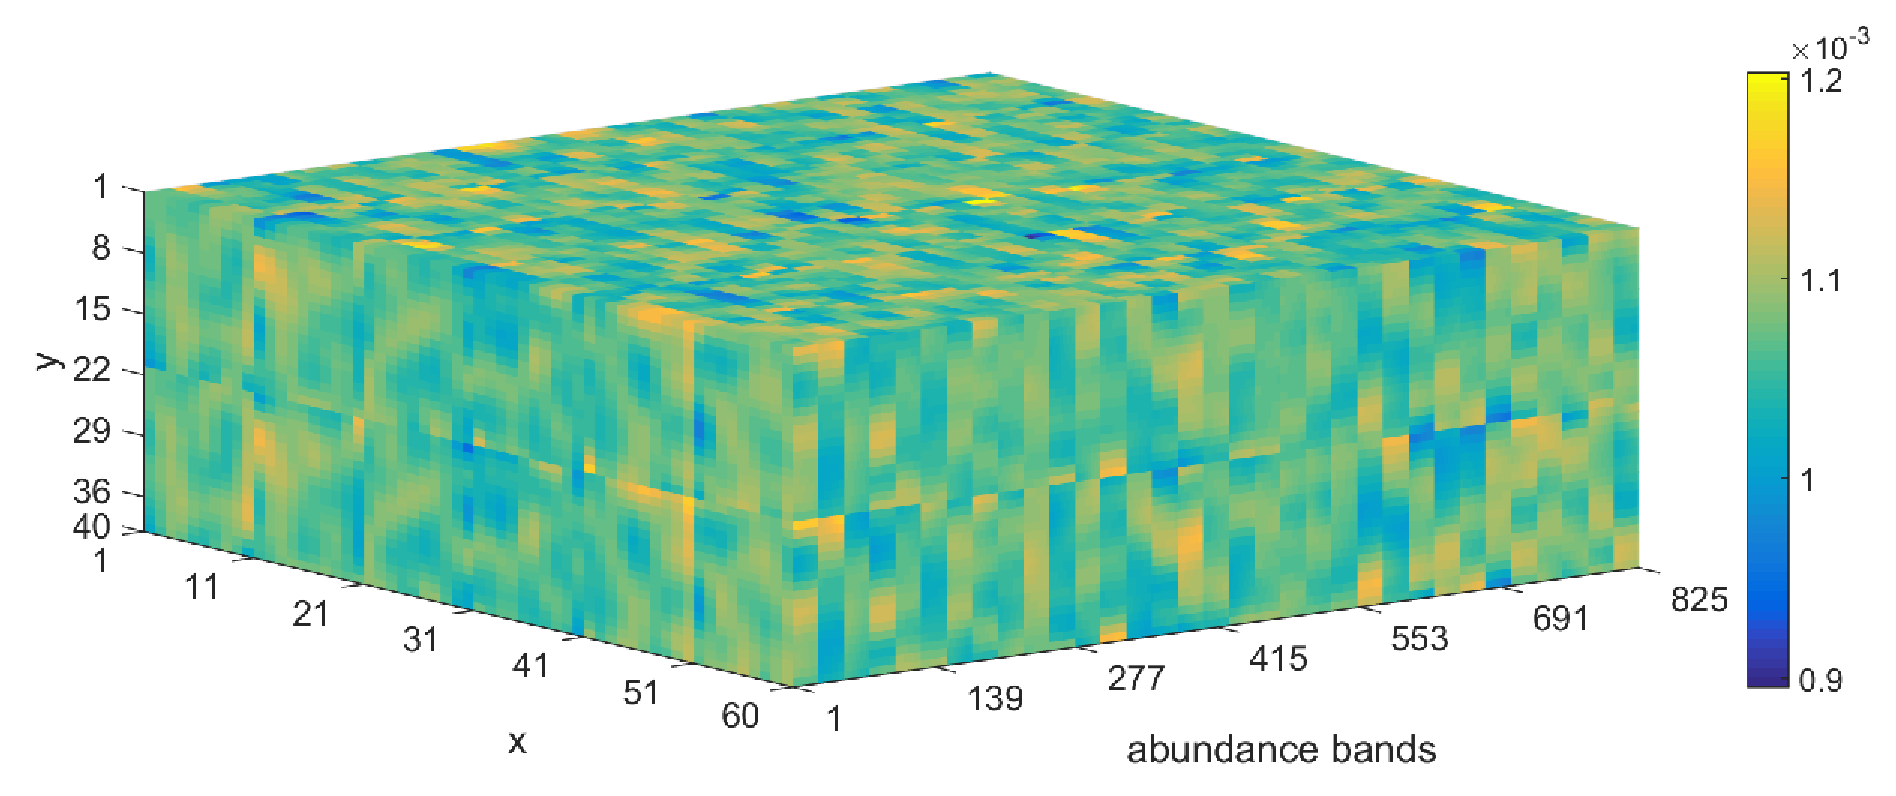
\includegraphics[height=\myheight]{./images/generated_A/3.eps}} \hspace{1mm} 
	\subfloat[d)]{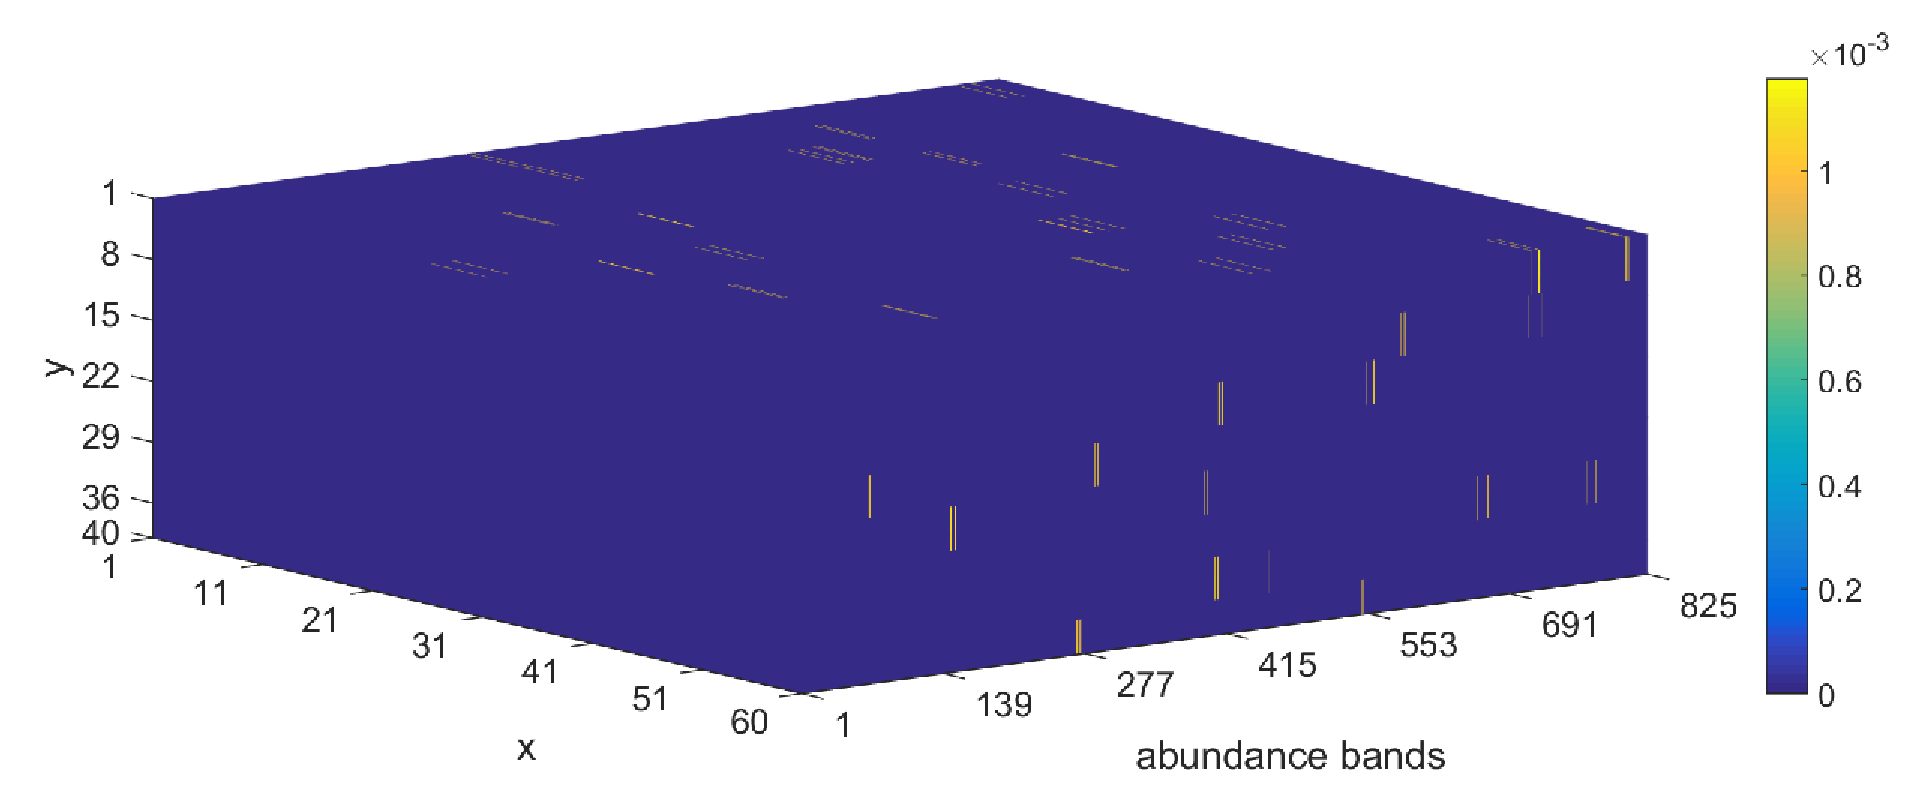
\includegraphics[height=\myheight]{./images/generated_A/4_A22.eps}} \hspace{1mm} 
	\caption{Steps for generating the synthetic ground truth abundance cubes. Spatial planes (frontal slices) are depicted with x and y axis, while in the  abundance direction, lateral slices are formed by abundance values for one x column and all y's. a) Uniformly generated abundance values, b) Spatially smoothed abundance values, c) Filtering in the abundance direction, d) Sparsity between and within groups of abundance values. In subfigure d), blue depicts non-active abundances, and yellow active abundances. }\label{genA}
\end{figure}
The parameter $\lambda$ was empirically selected between the range: $[10^{-5} - 1]$.
 
\subsection{Quantitative and qualitative results}
Our method was compared against a number of sparse unmixing approaches: SunSAL \cite{spUnmix} that considers sparsity over the abundance vector, SunSAL\_TV \cite{totVar}, that takes into account  spatial similarities between the abundances, CLSunSAL \cite{iordache14} accounting for joint sparsity between all the pixels sharing the same active set of endmembers and GSunSAL \cite{spGroup_unmix} containing within group and between group sparsity using multiple endmembers per group. The quality of the estimated abundances was assessed using the SRE performance metric: $SRE \equiv 20\log_{10}(\|\bA \|_2^2$ / $\|\bA -\hat{\bA} \|_2^2)$, with higher $SRE$ values meaning better unmixing. %$SRE \equiv 10\log_{10}(\frac{\|\bA \|_2^2}{\|\bA -\hat{\bA} \|_2^2})$ .
The $SRE$ results obtained from all methods are summarized in Table: \ref{sreTable}. One can notice that the $SRE$ values from our method are higher than the ones obtained from the other methods for all 4 synthetic data cubes. Moreover, qualitative results from the abundance maps for group 20 are shown in figure \ref{abunMaps}. Remark that the available set of abundance maps per group were averaged out in order to produce one abundance map per group. We can notice from this figure that our method produces a better reconstruction of the abundance map compared to the other techniques and copes better with the (local) smoothness of the abundance values in the spatial direction.  On the other side, due to the local smoothing, the map contains more non-zero values  at places where there are no active abundances, a price which has to be paid for simultaneously considering the (local) spatial homogeneity and  contributions from groups and elements within the groups. Yet, as opposed to the SunSAL\_TV which takes the spatial homogeneity over the entire area into account and thus oversmooths the abundance map(s), our method is able to deal better with the local spatial similarity, since we take only a spatial neighbourhood into account and not the entire area. In addition, a lateral slice of the abundance cube composed from abundance values for the last x column and all y rows from the cube is depicted in figure \ref{spec_abun_bands}. %across the abundance direction are depicted in figure \ref{spec_abun_bands}. 
We can see that the abundance map from our method follows more closely the ground truth map compared to the other techniques, with exception to the GSunSAL method with which it has the closest visual appearance. We can observe here that methods that take groups into account, as our method and the GSunSAL method, have some  \textit{leakage} of their abundance values within the group. Whenever a group is active, the \textit{leakage} is manifested as active/non-zero abundance values for endmember elements from the same group which are not suppose to be contributing to the mixed spectra.   
\begin{table*}[h!]
 \centering
    \caption{SRE values for 4 synthetic data cubes}
	\small
	\scalebox{0.85}{
    \begin{tabular}{|c|c|c|c|c|}
      						   \hline
            SNR = 20           &  Cube1 & Cube2 & Cube3 & Cube4\\
     						   \hline
     		NCLS               & $\mathbf{-0.6192}$        & $\mathbf{-1.6461}$ & $\mathbf{-1.7113}$ & $\mathbf{-4.1193}$   \\	
     		                   \hline	   
     		SunSAL             & $\mathbf{0.0114}$              & $\mathbf{-0.0241}$      & $\mathbf{-0.0096}$           & $\mathbf{-0.0306}$   \\
     		                   &($\lambda = 5\times10^{-4}$)  & ($\lambda = 10^{-3}$)   & ($\lambda = 5\times10^{-5}$) & ($\lambda = 10^{-3}$)   \\
     		                   \hline
			CLSunSAL           & $\mathbf{0.0504}$             & $\mathbf{0.0545}$             & $\mathbf{0.0475}$      & $\mathbf{0.0416}$   \\
			                   &($\lambda = 5\times10^{-4}$)   & ($\lambda = 5\times10^{-3}$)  & ($\lambda = 10^{-3}$)  & ($\lambda = 10^{-2}$)    \\
			                   \hline
			GSunSAL            & $\mathbf{0.1165}$        & $\mathbf{0.1914}$        & $\mathbf{0.1104}$        & $\mathbf{0.1693}$  \\
			                   &($\lambda = 10^{-5}$)     & ($\lambda = 10^{-5} $)   & ($\lambda = 10^{-5} $)   & ($\lambda = 10^{-5}$)   \\
			                   &($\lambda_g = 10^{-5} $)  & ($\lambda_g = 10^{-5} $) & ($\lambda_g = 10^{-5} $) & ($\lambda_g = 10^{-5} $)   \\
			                   \hline
			SunSAL\_TV         &  $\mathbf{0.0183}$ &  $\mathbf{0.0222}$ &  $\mathbf{0.0187}$  &  $\mathbf{0.0336}$ \\
			                   &($\lambda = 5\times 10^{-4}$)     & ($\lambda = 10^{-5} $)               & ($\lambda = 10^{-5} $)      & ($\lambda = 10^{-5}$)   \\
			                   &($\lambda_{TV} = 10^{-4} $)       & ($\lambda_{TV} = 5 \times 10^{-3} $) & ($\lambda_{TV} = 10^{-3} $) & ($\lambda_{TV} = 5\times 10^{-3} $)   \\
			                   \hline
			G\_Nuclear         &  $\mathbf{0.1389}$  &  $\mathbf{0.2254}$  &  $\mathbf{0.1221}$   &  $\mathbf{0.1907}$   \\
			                   &($\lambda = 10^{-5}$)  & ($\lambda = 10^{-5}$) & ($\lambda = 10^{-5}$) & ($\lambda = 10^{-4}$)    \\
			                   \hline
    %  	\bottomrule
    \end{tabular}
    }
%   \end{adjustbox}
 % \end{center}
 \label{sreTable}
\end{table*}
\begin{figure*}[h!]
	\captionsetup[subfigure]{labelformat=empty,font=small}
	\settoheight\myheight{\includegraphics[width=0.25\textwidth]{./images/abun_maps/Cube4JetG20/GroundTruth20.eps}}
	\centering
	\subfloat[a) Ground Truth]{\includegraphics[height=\myheight]{./images/abun_maps/Cube4JetG20/GroundTruth20.eps}} \hspace{1mm} 
	\subfloat[b) G. Nuclear]{\includegraphics[height=\myheight]{./images/abun_maps/Cube4JetG20/GroupNuclear20.eps}} \hspace{1mm} 
	\subfloat[c) GSunSAL]{\includegraphics[height=\myheight]{./images/abun_maps/Cube4JetG20/GSunSAL20.eps}} \hspace{1mm} 
	\subfloat[d) SunSAL\_TV]{\includegraphics[height=\myheight]{./images/abun_maps/Cube4JetG20/SunSALTV20.eps}} \hspace{1mm} 
	\subfloat[e) CLSunSAL]{\includegraphics[height=\myheight]{./images/abun_maps/Cube4JetG20/CLSunSAL20.eps}} \hspace{1mm}
	\subfloat[f) SunSAL]{\includegraphics[height=\myheight]{./images/abun_maps/Cube4JetG20/SunSAL20.eps}} \hspace{1mm}
	\caption{Spatial plane of abundance maps from group 15} \label{abunMaps}
\end{figure*}
\begin{figure*}[h!]
	\captionsetup[subfigure]{labelformat=empty,font=small}
	\settoheight\myheight{\includegraphics[width=0.25\textwidth]{./images/spectral_abun_Planes/Cube4/GT/rows_all_cols_end_abun_all.eps}}
	\centering
	\subfloat[a) Ground Truth]{\includegraphics[height=\myheight]{./images/spectral_abun_Planes/Cube4/GT/rows_all_cols_end_abun_all.eps}} \hspace{1mm} 
	\subfloat[b) G. Nuclear]{\includegraphics[height=\myheight]{./images/spectral_abun_Planes/Cube4/Nuclear/rows_all_cols_end_abun_all.eps}} \hspace{1mm} 
	\subfloat[c) GSunSAL]{\includegraphics[height=\myheight]{./images/spectral_abun_Planes/Cube4/GSUNSAL/rows_all_cols_end_abun_all.eps}} \hspace{1mm} 
	\subfloat[d) SunSAL\_TV]{\includegraphics[height=\myheight]{./images/spectral_abun_Planes/Cube4/SunSAL_TV/rows_all_cols_end_abun_all.eps}} \hspace{1mm} 
	\subfloat[e) CLSunSAL]{\includegraphics[height=\myheight]{./images/spectral_abun_Planes/Cube4/CLSunSAL/rows_all_cols_end_abun_all.eps}} \hspace{1mm}
	\subfloat[f) SunSAL]{\includegraphics[height=\myheight]{./images/spectral_abun_Planes/Cube4/SunSAL/rows_all_cols_end_abun_all.eps}} \hspace{1mm}
	\caption{Abundance maps across the abundance direction, i.e. lateral slice formed by the abundance values for the last x column and all y rows from the abundance cube.  }\label{spec_abun_bands} %
\end{figure*}
\section{Conclusions}
In this work, we proposed a sparse unmixing method with a group nuclear norm regularization, 
exploring the potential of the low rank structure of the abundances from neighboring pixels associated 
to endmembers from the same group. The advantage of this method is that it is  able to use the available information from multiple endmembers belonging to a group, capture the group information w.r.t. to the abundances, enforce sparsity between and withing these groups, and at the same time deal with (local) spatial similarity by using only one regularizer.  
From the experimental results, it can be  observed that our approach gives improved unmixing results, compared to the other methods, with relatively close values to GSunSAL, the method which takes group information in a independent way into account, but lacks inclusion of spatial information. Further topic of research would be to experiment with real hyperspectral scenes in order to demonstrate the contributions of our proposed method.
% -------------------------------------------------------------------------
\bibliographystyle{IEEEbib}
%\bibliography{bib}
\bibliography{refs}
\end{document}
